% Sgr A* Scientific Simulator — thesis / research report (paper/THESIS_PLAN.md).
% Compile: make thesis   (pdflatex ×3 + bibtex; numbers.tex and figures/ are
% auto-generated — every quantitative statement that is not a cited literature
% value comes from a \newcommand in numbers.tex, regenerated by
% `make reproduce`). The 11-page journal version is paper/main.tex (mnras);
% this document is the long-form report and shares numbers/figures/refs.
\documentclass[11pt,a4paper]{report}

\usepackage[a4paper,margin=2.6cm]{geometry}
\usepackage{amsmath}
\usepackage{amssymb}
\usepackage{graphicx}
\usepackage{booktabs}
\usepackage[round]{natbib}
\usepackage[hidelinks]{hyperref}

\setcounter{tocdepth}{2}   % contents lists chapters, sections, subsections
\setcounter{secnumdepth}{2}

% AUTO-GENERATED by scripts/make_numbers.py — do not edit by hand.
% Regenerate with `make reproduce` / `py -3.11 scripts/make_numbers.py`.
\newcommand{\FitMass}{4.270}
\newcommand{\FitMassErr}{0.195}
\newcommand{\FitDist}{8272}
\newcommand{\FitDistErr}{182}
\newcommand{\FitSma}{124.82}
\newcommand{\FitSmaErr}{0.88}
\newcommand{\FitEcc}{0.88277}
\newcommand{\FitEccErr}{0.00195}
\newcommand{\FitIncl}{134.70}
\newcommand{\FitInclErr}{0.41}
\newcommand{\FitOmegaBig}{227.33}
\newcommand{\FitOmegaBigErr}{0.63}
\newcommand{\FitOmegaSm}{65.44}
\newcommand{\FitOmegaSmErr}{0.61}
\newcommand{\FitTPeri}{2002.3227}
\newcommand{\FitTPeriErr}{0.0052}
\newcommand{\FitPeriod}{16.0561}
\newcommand{\FitPeriodErr}{0.0228}
\newcommand{\FitChiTwo}{307.8}
\newcommand{\FitDof}{321}
\newcommand{\FitChiRed}{0.959}
\newcommand{\FitNAst}{145}
\newcommand{\FitNRv}{44}
\newcommand{\GrExcessPeak}{205}
\newcommand{\GrExcessEpoch}{2018.379}
\newcommand{\PrecSchw}{11.98}
\newcommand{\PrecLT}{-0.204}
\newcommand{\FitMassNSigma}{0.14}
\newcommand{\FitDistNSigma}{0.03}
\newcommand{\EpsQBest}{0.00}
\newcommand{\EpsQSigma}{0.93}
\newcommand{\EpsQCiNinetyFive}{1.33}
\newcommand{\EpsQForecastTenOrbits}{0.34}
\newcommand{\SchwDiamM}{10.3924}
\newcommand{\SchwSpreadPct}{0.000}
\newcommand{\KerrDiamM}{9.5445}
\newcommand{\KerrDiamUas}{48.91}
\newcommand{\BeamRatio}{9.60}
\newcommand{\GMin}{0.139}
\newcommand{\GMax}{1.440}
\newcommand{\FluxRatioZeroOne}{10.7}
\newcommand{\FluxRatioOneTwo}{274}
\newcommand{\CalDiamUas}{49.68}
\newcommand{\CalDiamM}{9.695}
\newcommand{\CalAxisRatio}{0.9946}
\newcommand{\UasPerM}{5.1243}
\newcommand{\GpuMeanDiff}{0.00289}
\newcommand{\GpuMaxDiff}{0.697}
\newcommand{\GpuOutliers}{32}
\newcommand{\BenchCpuNullStepsPerS}{1,340,753}
\newcommand{\BenchCpuChristoffelPerS}{508,369}
\newcommand{\BenchCpuTimelikeStepsPerS}{78,987}
\newcommand{\BenchGpuFpsHd}{47.5}
\newcommand{\BenchGpuFpsFullhd}{21}
\newcommand{\BenchGpuMegaraysPerSHd}{43.8}
\newcommand{\EtaSchw}{5.72}
\newcommand{\EtaSgrA}{17.96}
\newcommand{\EtaNearExtremal}{32.10}
\newcommand{\GammaPolarSgrA}{2.571}
\newcommand{\GammaProSgrA}{3.142}
\newcommand{\GammaRetroSgrA}{3.142}
\newcommand{\ProjOnWorstDev}{9.6\times10^{-12}}
\newcommand{\ProjOffWorstPct}{93}
\newcommand{\ProjOffBestDev}{1.1\times10^{-04}}
\newcommand{\SubringRatioZeroOneLo}{8.6}
\newcommand{\SubringRatioZeroOneHi}{16.8}


% Shorthand (shared with main.tex)
\newcommand{\muas}{\mu\mathrm{as}}
\newcommand{\msun}{\mathrm{M}_\odot}
\newcommand{\sgra}{Sgr~A*}
\newcommand{\astar}{a_*}
\newcommand{\epsq}{\varepsilon_q}

% Stub marker used while chapters are under construction
\newcommand{\stub}[1]{\begin{quote}\itshape [Chapter under construction —
scope: #1 See \texttt{paper/THESIS\_PLAN.md}.]\end{quote}}

\begin{document}

% Front matter: cover page (page 1), contents (page 2+), abstract, notation,
% reproducibility statement.

%---------------------------------------------------------------- cover page
\begin{titlepage}
\centering
\vspace*{1.2cm}
{\Huge\scshape S\,G\,R\ \ A*\par}
\vspace{0.5cm}
{\LARGE A First-Principles Relativistic Simulator of the\\
Galactic-Centre Black Hole\par}
\vspace{0.9cm}
{\large Shadow metrology, S-star orbit fitting, and a free-quadrupole\\
test of the no-hair theorem — with a complete account of the\\
methods, tests, and development of the instrument\par}
\vspace{1.4cm}
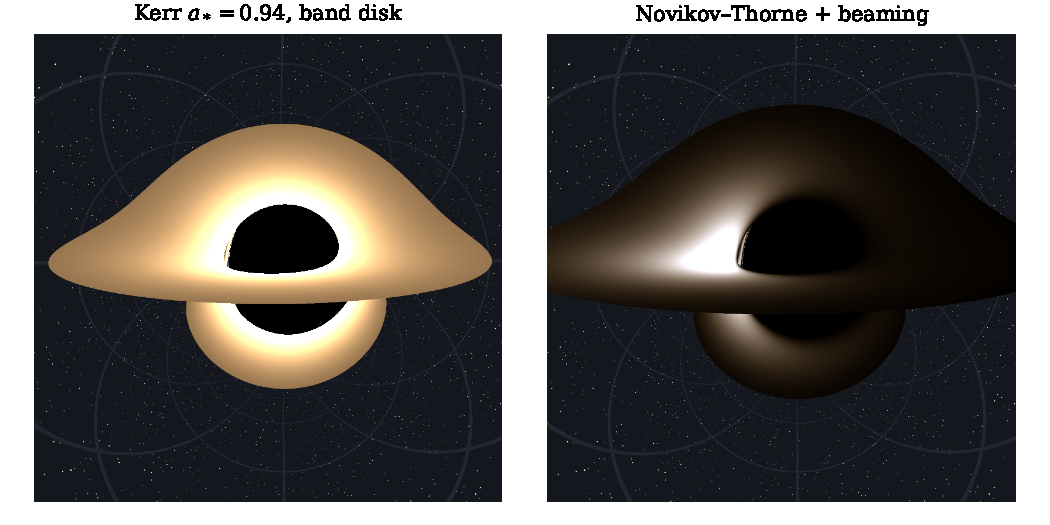
\includegraphics[width=0.82\textwidth]{figures/fig_disk_render.pdf}
\vfill
{\large C.~Excelsis\par}
\vspace{0.3cm}
{\large Independent research report\par}
\vspace{0.3cm}
{\large \today\par}
\end{titlepage}

%---------------------------------------------------------------- contents
\pagenumbering{roman}
\tableofcontents
\listoffigures
\listoftables
\cleardoublepage

%---------------------------------------------------------------- abstract
\chapter*{Abstract}
\addcontentsline{toc}{chapter}{Abstract}

We present a ground-up, physically rigorous simulator of the Galactic-centre
black hole \sgra{}, built on exact Kerr geodesics and validated end-to-end
against published strong-field observations. Null and timelike geodesics are
integrated in a second-order Mino-time formulation of the Carter equations
with per-step constraint projection, conserving $(E, L_z, Q)$ to better than
$10^{-6}$ relative over complete orbits. A CPU reference ray tracer
reproduces the analytic Schwarzschild shadow to a relative accuracy of
$5\times10^{-16}$ and the Bardeen critical curve for spinning holes; a
double-precision GPU compute port agrees with the CPU ground truth to a mean
pixel residual of \GpuMeanDiff. Fitting 13 orbital and potential parameters
to the \FitNAst{} astrometric and \FitNRv{} radial-velocity measurements of
the star S2 \citep{Gillessen2017} with full general-relativistic timelike
geodesics recovers $M = \FitMass \pm \FitMassErr \times 10^{6}\,\msun$ and
$R_0 = \FitDist \pm \FitDistErr$~pc, within $\FitMassNSigma\sigma$ and
$\FitDistNSigma\sigma$ of the GRAVITY interferometric values, at a reduced
$\chi^2$ of \FitChiRed. The model reproduces the gravitational-redshift
excess at the 2018 pericentre passage
($\GrExcessPeak\,\mathrm{km\,s^{-1}}$ peak) detected by
\citet{Gravity2018}, and the Schwarzschild precession of
$\PrecSchw$~arcmin per orbit confirmed by \citet{Gravity2020}. At the
GRAVITY mass and distance the simulated photon ring diameter is
$\CalDiamUas\,\muas$, inside the EHT measurement of
$51.8\pm2.3\,\muas$ \citep{EHT2022}. Freeing the quadrupole moment in a
Hartle--Thorne extension yields
$\epsq = \EpsQBest \pm \EpsQSigma \times 10^{5}$ (68 per cent),
consistent with the no-hair theorem.

This report is the long-form account of that programme. Part~I is a
plain-language primer for readers without a physics background. Parts~II--IV
derive, from first principles, every formula the simulator implements;
document the numerical methods and their error analysis; present the full
results with their statistical treatment; and record the complete
development history, test suite, and validation gates through which the
instrument was built.

% TODO(thesis): expand to ~400 words when the MCMC and cluster-fit results land.

%---------------------------------------------------------------- notation
\chapter*{Notation and Conventions}
\addcontentsline{toc}{chapter}{Notation and Conventions}

Geometric units $G=c=1$ are used throughout unless stated; masses, lengths
and times are quoted in units of the gravitational radius $M$
(for \sgra{}: $GM/c^2 = \UasPerM^{-1}$ scaling on the sky, $GM/c^3 = 21.17$~s).
Metric signature $(-,+,+,+)$; Boyer--Lindquist coordinates
$(t,r,\theta,\phi)$.

% TODO(thesis): full symbol table (M, a, a*, Sigma, Delta, A, E, Lz, Q, mu,
% lambda Mino, tau, eps_q, g, xi, eta, gamma_Lyapunov, chi2, ...).

%------------------------------------------------- reproducibility statement
\chapter*{Reproducibility Statement}
\addcontentsline{toc}{chapter}{Reproducibility Statement}

Every quantitative statement in this report that is not a cited literature
value is typeset from a macro in \texttt{numbers.tex}, generated by
\texttt{scripts/make\_numbers.py} from machine-readable artefacts produced by
the simulation; every figure is generated by \texttt{make figures}
(matplotlib) from the same artefacts. The single command
\texttt{make reproduce} re-runs the full chain — unit tests, reference
renders, sub-ring metrology, orbit fits, calibration, sweeps, and figure
generation — from source. A number that cannot survive this cycle cannot
appear in this document.

\cleardoublepage
\pagenumbering{arabic}


%======================================================================
\part{Foundations for the Non-Specialist}
\chapter{Gravity, Mass, and the Idea of a Black Hole}
\label{ch:f1}

\noindent\emph{This first part of the report assumes no physics background at
all. It explains, in ordinary language, every idea the technical chapters
build on. If you are comfortable with general relativity, skip directly to
Part~II.}

\section{Throwing things upward}

Throw a ball into the air and it comes back. Throw it harder and it climbs
higher before it comes back. This everyday fact hides a precise question:
\emph{is there a throwing speed so great that the ball never comes back at
all?}

There is. For every planet or star there is a special speed, the
\emph{escape velocity}, at which a thrown object just barely coasts away
forever, slowing all the while but never quite stopping. From the surface of
the Earth it is about 11~kilometres per second — thirty times the speed of
sound. From the surface of the Sun it is about 620 kilometres per second.
The rule of thumb is simple: the more mass squeezed below you, and the
closer you stand to it, the faster you must go to leave.

\begin{worked}{How fast must you throw?}
The escape velocity has a one-line recipe. A thrown object escapes if
its energy of motion, $\tfrac12 v^2$ for every kilogram of it, at least
matches the energy needed to climb out of the gravity well, $Gm/r$ per
kilogram — where $m$ is the planet's mass, $r$ its radius, and $G$ is
Newton's gravitational constant, $6.67\times10^{-11}$ in SI units.
Setting the two equal and solving for $v$:
\[
v_{\rm esc}=\sqrt{\frac{2Gm}{r}}.
\]
For the Earth, $m = 5.97\times10^{24}$~kg and $r = 6\,371$~km, so
$2Gm = 7.97\times10^{14}$~m$^3$/s$^2$; dividing by
$r = 6.371\times10^{6}$~m gives $1.25\times10^{8}$~m$^2$/s$^2$, and the
square root is $11\,200$~m/s — the 11~km/s quoted above. Notice that
nothing in the formula cares what the ball is made of: only total mass
and radius enter. That indifference is the loophole a black hole
exploits.
\end{worked}

That second part — \emph{the closer you stand} — is the key to everything
in this report. Squeeze the same mass into a smaller ball and its surface
moves closer to the centre, so the escape velocity from that surface goes
up, even though the total mass never changed. Squeeze the Sun to a radius of
three kilometres and the escape velocity at its surface would reach the
fastest speed there is: the speed of light, about
300\,000~kilometres per second.

\section{The point of no return}

Light's speed is not just fast; physics as we understand it (and as
Chapter~\ref{ch:f2} sketches) says nothing can move faster. So an object
compressed within that critical size has a startling property: at some
radius, not even light travels fast enough to escape. Whatever falls inside
can send no signal out. The sphere where escape would require exactly the
speed of light is called the \emph{event horizon}: an ``event'' happening
inside it can never be seen from outside, even in principle.

An object like this is a \emph{black hole} — black because no light leaves
it, and a hole because things can fall in but not climb out. The critical
radius is named the \emph{Schwarzschild radius} after Karl Schwarzschild,
who solved Einstein's equations for a single round mass within weeks of
their publication in 1915. The Schwarzschild radius grows in direct
proportion to the mass: double the mass and the horizon doubles in size.
For the Earth it is about nine millimetres — the Earth would have to be
crushed to the size of a marble. For the Sun, about three kilometres. For
the black hole at the centre of our Galaxy, which weighs about 4.3 million
Suns, it is around 13 million kilometres — some eighteen times the radius
of the Sun, yet still tiny on galactic scales.

Two cautions about the picture this conjures. First, the horizon is not a
surface you could touch: nothing is \emph{there}. It is a boundary drawn in
empty space, the line on the map beyond which no path leads back out. A
falling astronaut would notice nothing special while crossing it. Second,
the mass is not spread throughout the dark sphere. As far as the theory can
say, everything that fell in is concentrated at the centre in a region
where the equations lose their meaning — the \emph{singularity}. The
singularity is a statement of ignorance rather than a physical prediction:
it marks where the current theory of gravity stops being trustworthy.
Fortunately, for everything in this report only the \emph{outside} of the
horizon matters, and there the theory is precise and testable.

\begin{worked}{The size of \sgra{}'s horizon}
Ask the escape-velocity recipe a pointed question: at what radius does
$v_{\rm esc}$ reach the speed of light? Set $v_{\rm esc}=c$ and solve
for the radius:
\[
R_S=\frac{2Gm}{c^2}.
\]
For \sgra{}, $m = 4.297$ million solar masses
$= 4.297\times10^{6}\times1.989\times10^{30}~{\rm kg}
= 8.55\times10^{36}$~kg. Then $2Gm = 1.14\times10^{27}$ in SI units,
and dividing by $c^2 = 9.0\times10^{16}$~m$^2$/s$^2$ gives
\[
R_S = 1.27\times10^{10}~{\rm m} \approx 12.7\ \hbox{million km},
\]
about eighteen Sun-radii, as quoted in the text; light itself would
need 42 seconds to cross that distance. One honest caution: we used
Newton's energy formula in a regime where Newton's theory fails. By a
happy algebraic coincidence the fully relativistic calculation
(Chapter~\ref{ch:kerr}) returns \emph{exactly} the same $R_S$ — which
is why this little derivation, essentially the one John Michell wrote
down in 1784, is worth showing at all.
\end{worked}

\section{Falling in: the gentle giant surprise}

One more everyday idea unlocks a real result. Stand on the Earth and
your feet are pulled slightly harder than your head — they are closer
to the centre. Near a compact mass this difference, the \emph{tidal}
force, can become violent: fall feet-first toward a small black hole
and the pull on your feet so exceeds the pull on your head that you
would be stretched like taffy (astrophysicists genuinely say
\emph{spaghettification}).

Here is the surprise: the bigger the black hole, the \emph{gentler}
its horizon. The tidal stretch across a falling body depends on the
mass divided by the \emph{cube} of the distance, and since the horizon
radius grows in proportion to the mass, the stretch \emph{at the
horizon} falls off as one over the mass squared. Crossing the horizon
of a 10-solar-mass black hole, the difference in pull across a
two-metre astronaut is about $2\times10^{8}$~m/s$^2$ — twenty million
times Earth's gravity, lethal long before arrival. Crossing the
horizon of \sgra{}, four hundred thousand times heavier, the same
difference is about one \emph{millimetre} per second squared — less
than the tug your feet feel from standing on a kerb. An astronaut
would drift across \sgra's point of no return without a twinge,
noticing nothing at all; the drama is reserved for much deeper in.
This is why nothing dramatic marks the horizon in the renders of this
report: general relativity says, correctly, that locally there is
nothing there (the caution of the previous section made precise).

\section{Sagittarius A*, our own giant}

Point a telescope at the constellation Sagittarius and you look toward the
centre of the Milky Way, 8\,277 parsecs away (a \emph{parsec} is about 3.26
light-years; the light arriving tonight left before the last ice age
peaked). At the exact dynamical centre sits a compact radio source named
\sgra{} (``Sagittarius A star''). Around it, stars swarm at extraordinary
speeds — a few pass their closest approach at several thousand kilometres
\emph{per second}, about a hundred times faster than the Earth orbits the
Sun. Something enormously heavy and enormously compact must be holding
them: the measured mass is $4.297\pm0.012$ million solar masses, packed
into a region smaller than the orbit of Mercury. No cluster of dim stars,
no exotic gas cloud survives scrutiny as an alternative; a supermassive
black hole is the only explanation standing
(Chapter~\ref{ch:intro} gives the observational history).

\sgra{} is the star of this report for a practical reason: it is the
\emph{nearest} supermassive black hole, and the only one where two entirely
different kinds of measurement meet. We can follow individual stars looping
around it year by year (Chapters~\ref{ch:f5}, \ref{ch:sstar},
\ref{ch:fitting}), and we can photograph the glowing ring of light bent
around its horizon (Chapters~\ref{ch:f3}, \ref{ch:shadow}). This report
describes a simulator built from first principles that reproduces both
kinds of measurement from the same underlying equations.

\section{A sense of scale}

The numbers in this subject span so many powers of ten that it is worth
pausing to place them on one line (Fig.~\ref{fig:dgscales}).

\begin{figure}
\centering
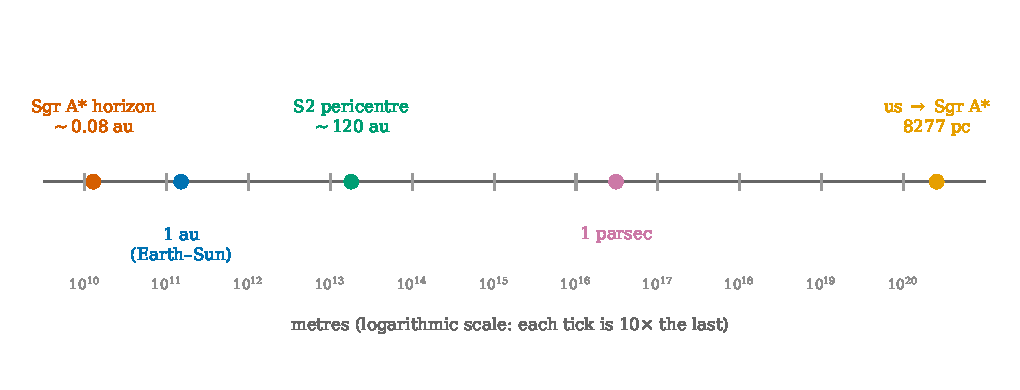
\includegraphics[width=\textwidth]{figures/dg_scales.pdf}
\caption{The scales of the problem on a single logarithmic line, from the
\sgra{} horizon to its distance from us. Each tick is ten times the
previous one: the distance to \sgra{} is about twenty billion times the
size of its horizon — comparable to viewing a coin at the distance of the
Moon.}
\label{fig:dgscales}
\end{figure}

Astronomers measure distances within a planetary system in
\emph{astronomical units} (au): one au is the Earth–Sun distance, about 150
million kilometres. The horizon of \sgra{} spans about a sixth of an
au. The star S2, the most important character of Part~III, dives to about
120~au from the black hole — about three times the distance of Pluto from
the Sun — which sounds close until you recall that this is still about
1\,500 horizon radii out.

For things on the sky, astronomers use angles. A degree is what your little
finger covers at arm's length; an \emph{arcsecond} is 1/3600 of a degree,
roughly a coin seen from four kilometres away; and the measurements in this
report are made in \emph{milliarcseconds} (a thousandth of an arcsecond)
and \emph{microarcseconds} ($\muas$, a millionth). The photon ring of
\sgra{} spans about 52~$\muas$ — the apparent size of a doughnut on the
Moon. That such an angle is measurable at all, by linking radio telescopes
across the whole Earth into one instrument, is among the technical wonders
of modern astronomy.

One more unit will keep appearing: the \emph{gravitational radius}, written
$M$ in this report. It is the natural yardstick of a black hole — half the
Schwarzschild radius — and it lets us describe any black hole, whatever
its mass, with the same numbers. ``The disk's inner edge sits at $6\,M$''
is true of a stellar black hole and of \sgra{} alike; only the metre-stick
changes. Chapter~\ref{ch:f6} says more about this trick of working in
natural units.

\begin{termsbox}
\item[Escape velocity] The launch speed at which an object barely coasts
away from a mass forever.
\item[Event horizon] The boundary around a black hole from inside which
nothing, not even light, can escape. Not a material surface.
\item[Schwarzschild radius] The size of the event horizon of a
non-spinning mass; proportional to the mass.
\item[Singularity] The central region where the known equations of gravity
break down; hidden inside the horizon.
\item[\sgra{}] The 4.3-million-solar-mass black hole at the centre of the
Milky Way, 8\,277 parsecs away.
\item[au, parsec, milli-/microarcsecond] Units for distances and sky
angles; see Fig.~\ref{fig:dgscales}.
\item[Gravitational radius ($M$)] The natural length unit of a black hole;
the horizon of a non-spinning hole sits at $2\,M$.
\end{termsbox}

\noindent$\rightarrow$ \emph{Full treatment: the observational case for
\sgra{} in Chapter~\ref{ch:intro}; the exact horizon formulas in
Chapter~\ref{ch:kerr}.}

\chapter{Spacetime and Einstein's Gravity, Gently}
\label{ch:f2}

\section{Gravity is not a pull}

Newton described gravity as a force: the Earth pulls the apple, the Sun
pulls the Earth. His description is astonishingly accurate for slow
objects far from big masses, and Chapter~\ref{ch:f5} will use it freely.
But it leaves a mystery — how does the Sun reach across empty space to
tug on the Earth? — and it fails, measurably, exactly in the situations
this report cares about.

Einstein's 1915 answer, \emph{general relativity}, removes the mystery by
removing the force. In his picture, mass does not pull on distant objects.
Instead, mass changes the shape of \emph{spacetime} — the four-dimensional
fabric of the three space directions plus time — in its neighbourhood, and
objects then simply travel through that reshaped fabric in the straightest
possible lines. The famous slogan, due to John Wheeler, is: \emph{matter
tells spacetime how to curve, and spacetime tells matter how to move.}

A useful (if imperfect) picture is a stretched rubber sheet with a bowling
ball resting in the middle. Marbles rolled across the sheet curve toward
the ball, not because the ball grips them, but because the surface they
travel on slopes. Each marble is doing the most natural thing possible —
going straight ahead on a surface that is not flat. The Earth orbits the
Sun for the same reason: it moves straight ahead through a region of
spacetime that the Sun has curved, and ``straight ahead'' there is a loop.

The straightest possible path through curved spacetime has a name that
appears on nearly every page of Part~II: a \emph{geodesic}. On the Earth's
curved surface, geodesics are the great circles that airliners follow; in
curved spacetime, geodesics are the paths of everything that falls freely
— thrown stones, orbiting planets, and light itself. The entire simulator
described in this report is, at its heart, a machine for computing
geodesics very accurately.

\section{Light bends}

Because light also travels through spacetime, its path also bends where
spacetime curves. The effect is tiny near the Sun — starlight grazing the
solar surface deflects by less than two arcseconds, first measured during
the 1919 eclipse — but near a black hole the bending becomes wild.

Fig.~\ref{fig:trajschw} shows real computed light paths around a
non-spinning black hole, calculated with the same equations the simulator
uses. A ray passing far away bends gently, like the starlight of 1919. A
ray passing closer bends more. And there is a critical aiming distance at
which the bending wins completely: the ray wraps around the hole and can
circle it — light in orbit. Aim any closer and the ray spirals in and is
gone. The dividing line between ``escapes, however bent'' and ``captured''
is what carves out the black-hole \emph{shadow}, the subject of
Chapter~\ref{ch:f3}.

\begin{figure}
\centering
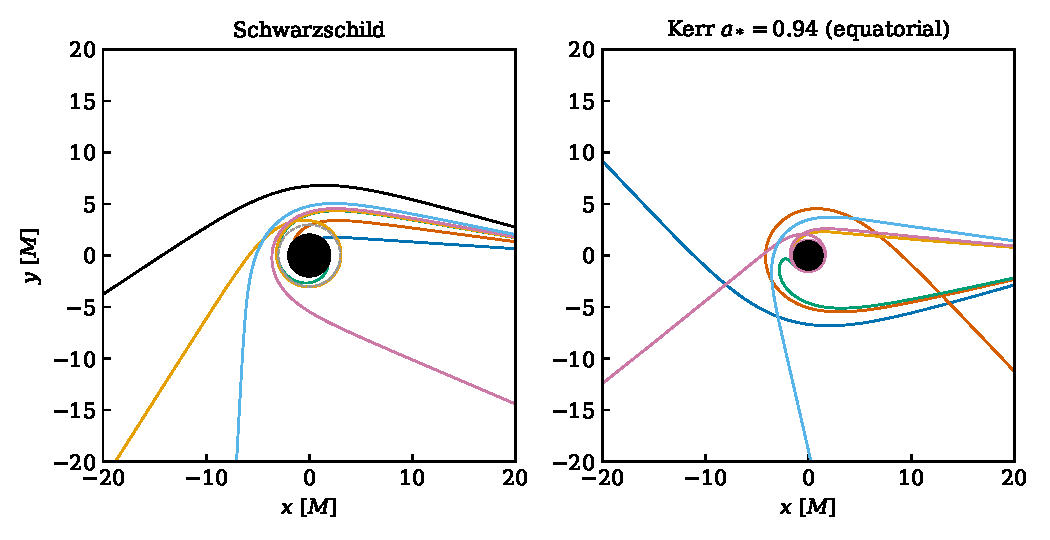
\includegraphics[width=\textwidth]{figures/fig_photon_trajectories.pdf}
\caption{Computed paths of light rays in the equatorial plane of a black
hole, from the simulator's own geodesic integrator. Left: a non-spinning
(Schwarzschild) hole — rays aimed farther out escape with a bend; a
critical ray circles on the dashed photon sphere; closer rays are
captured. Right: a rapidly spinning (Kerr) hole — the spacetime itself
circulates, so rays travelling with the spin behave differently from rays
travelling against it (Chapter~\ref{ch:f3}).}
\label{fig:trajschw}
\end{figure}

This bending also acts as a distorting lens. A black hole with a glowing
disk around it shows you the disk twice over: light from the part of the
disk hidden \emph{behind} the hole is bent up and over the top (and under
the bottom), so the far side appears above and below the dark centre. That
is why the famous images — the Event Horizon Telescope's photographs and
the film \emph{Interstellar}'s Gargantua — have their characteristic
crossed-halo look. Every one of those features appears, for the right
physical reasons, in the renders of Part~III.

\begin{worked}{The 1919 deflection, in two lines}
General relativity gives a compact formula for the bending of a light
ray that passes a mass $m$ at closest distance $r$ (it follows from the
same equations the simulator integrates, Chapter~\ref{ch:geodesics}):
\[
\delta = \frac{4Gm}{c^2 r}.
\]
The combination $Gm/c^2$ — a mass expressed as a length — will follow
us through the whole report; for the Sun it is $1.48$~km. A ray grazing
the solar surface has $r = 696\,000$~km, so
$\delta = 4\times1.48/696\,000 = 8.5\times10^{-6}$~radians. Multiplying
by $206\,265$ (arcseconds per radian) gives $1.75''$ — precisely the
deflection Eddington's expeditions went to measure in 1919, and double
what a na\"ive Newtonian calculation predicts. The factor of two is
pure spacetime curvature: half the bend comes from time running slow,
half from space itself being curved.
\end{worked}

\section{Time runs slow near mass}

Curved spacetime does something with no Newtonian counterpart at all: it
changes the rate of time. Clocks deeper in a gravitational well genuinely
run slower as seen from outside — not because of any mechanical fault, but
because ``one second'' is itself a local quantity, like ``north'', that
depends on where you are.

The effect is real and routine: the satellites of the GPS system carry
clocks about 20\,000~km above the Earth, where time runs faster than at
the ground by about 45 microseconds per day. Uncorrected, satellite
navigation would drift by kilometres within a day. Near a black hole the
same effect grows enormous; at the horizon, an outside observer would see
a falling clock slow to a stop.

\begin{worked}{The GPS correction, by the numbers}
The fractional rate difference between a clock at radius $r_1$ and one
at radius $r_2$ is, to an excellent approximation,
$(Gm/c^2)\,(1/r_1 - 1/r_2)$. For the Earth,
$Gm/c^2 = 4.4$~\emph{millimetres} — the Earth's mass written as a
length. With the ground at $r_1 = 6\,371$~km and the GPS orbit at
$r_2 = 26\,560$~km:
\[
\frac{1}{r_1}-\frac{1}{r_2} = 1.19\times10^{-7}~{\rm m}^{-1},
\qquad
0.0044\times1.19\times10^{-7} = 5.3\times10^{-10}.
\]
Multiply by the $86\,400$ seconds in a day: $46$ microseconds — the
satellite clocks run \emph{fast} by that much, because they sit higher
in the well. (Special relativity's time dilation from orbital speed
works the other way and claws back about $7\,\mu$s, for a net
$39\,\mu$s a day.) Light travels twelve kilometres in $39\,\mu$s:
ignore relativity today and satellite navigation is off by kilometres
by tomorrow.
\end{worked}

For this report the significance is very concrete: when the star S2 dives
to its closest approach to \sgra{}, its light is emitted from slightly
deeper in the black hole's gravitational well, where time runs slower.
Every wave of its light is stretched on the climb out — the wavelength
shifts toward the red. The GRAVITY instrument measured exactly this
\emph{gravitational redshift} in 2018, and reproducing that measurement
from first principles is one of this report's central results
(Chapters~\ref{ch:f4}, \ref{ch:fitting}).

\begin{worked}{S2's slowed clock, on an envelope}
How large is the effect for S2 at closest approach? The fractional
redshift of light climbing out from radius $r$ is roughly $Gm/(c^2 r)$.
For \sgra{}, $Gm/c^2 = 6.35\times10^{9}$~m — half the horizon radius
computed in Chapter~\ref{ch:f1} — and S2's closest approach is
$r \approx 120~{\rm au} = 1.80\times10^{13}$~m:
\[
z_{\rm grav} \approx \frac{6.35\times10^{9}}{1.80\times10^{13}}
= 3.5\times10^{-4}.
\]
A wavelength stretch of $3.5\times10^{-4}$ masquerades, in a
spectrograph, as an extra recession speed of
$3.5\times10^{-4}\times c \approx 106$~km/s. That — about a hundred
km/s of ``impossible'' extra redshift, switching on only around closest
approach — is the size of the signal GRAVITY hunted in 2018, and
Chapter~\ref{ch:fitting} shows our full model reproducing it with no
adjustable amplitude.
\end{worked}

\section{How we know: a century of passed tests}

It is fair to ask why anyone trusts this theory enough to build a
thesis on it. The answer is a hundred years of passed examinations,
each sharper than the last. The 1919 eclipse measurement of bent
starlight (worked above) made the theory famous; the anomalous
43-arcseconds-per-century creep of Mercury's orbit — known and
unexplained for six decades before Einstein — was retro-dicted
exactly, with no adjustable constant. The twentieth century added
laboratory redshift measurements (light climbing a 22-metre tower in
1959), the slowing of radar echoes grazing the Sun, and the patient
20\,000-fold-verified spin-down of the Hulse--Taylor binary pulsar,
which loses orbital energy at precisely the rate gravitational-wave
emission predicts. The twenty-first century has heard those waves
directly (LIGO, 2015) and photographed photon rings (EHT, 2019 and
2022). Every test in this list interrogates a different limb of the
theory — weak field, strong field, static, dynamical — and none has
ever returned a confirmed violation. The measurements this report
reproduces (the S2 redshift and precession, the ring diameter) are
the newest entries in that ledger, and the no-hair test of
Chapter~\ref{ch:nohair} is an attempt to \emph{add} one: the point of
precision reproduction is to build apparatus wherever the theory
could still fail.

\section{What a metric is (without tensors)}

One piece of vocabulary unlocks all of Part~II. To compute anything, we
need coordinates — labels like latitude and longitude that name the points
of spacetime. But coordinates are just names; they do not tell you how
\emph{far apart} two nearby points really are. On the Earth, one degree of
longitude is 111~km at the equator and zero at the pole: the conversion
from coordinate differences to true distances varies from place to place.

The rulebook for that conversion is called the \emph{metric}. Give the
metric the small coordinate steps between two nearby events (a bit of
north--south, a bit of east--west, a bit of time) and it returns the true
separation — including the true amount of elapsed clock time. All of the
curvature of spacetime is encoded in how this rulebook changes from place
to place; slow-running clocks and bending light are both just entries in
the rulebook. Einstein's field equations determine the metric produced by
a given arrangement of mass; for a lone spinning black hole the exact
answer is known and is the famous \emph{Kerr metric}
(Chapters~\ref{ch:f3}, \ref{ch:kerr}), on which this entire simulator is
founded.

When Part~II writes symbols such as $g_{tt}$ or $g_{r r}$, nothing deeper
is meant than ``the entry of the rulebook that converts time-steps (or
radius-steps) into true separations, at this location''.

\begin{termsbox}
\item[Spacetime] Space and time treated as one four-dimensional fabric,
whose shape is what we experience as gravity.
\item[General relativity (GR)] Einstein's theory: mass curves spacetime;
freely falling objects follow the straightest paths in it.
\item[Geodesic] The straightest possible path through curved spacetime;
the track of anything falling freely, including light.
\item[Gravitational lensing] The bending of light by curved spacetime; a
black hole shows the far side of its own disk, bent over the top.
\item[Time dilation] Clocks deeper in a gravitational well run slower;
measurable with GPS satellites and with the star S2.
\item[Gravitational redshift] Light climbing out of a gravitational well
is stretched to longer, redder wavelengths.
\item[Metric] The location-dependent rulebook that converts coordinate
differences into true distances and times; in GR it carries all of
gravity.
\end{termsbox}

\noindent$\rightarrow$ \emph{Full treatment: the Kerr metric in
Chapter~\ref{ch:kerr}; geodesics and their conserved quantities in
Chapter~\ref{ch:geodesics}; the traced light-bending figures in
Chapters~\ref{ch:geodesics} and \ref{ch:shadow}.}

\chapter{Spinning Black Holes and the Shadow}
\label{ch:f3-spin-shadow}

\stub{Kerr vs Schwarzschild, frame dragging, the ergosphere, the photon sphere, and how the shadow forms.}

\chapter{Light, Heat, and Colour: Reading the Disk}
\label{ch:f4-light-colour}

\stub{blackbody colour, the accretion disk, Doppler beaming, and the three redshifts.}

\chapter{Orbits, S-Stars, and Weighing a Black Hole}
\label{ch:f5-orbits}

\stub{Kepler's ellipse, astrometry vs radial velocity, precession, and how mass and distance emerge.}

\chapter{The Toolkit in Plain Words}
\label{ch:f6-toolkit}

\stub{geometric units, tensors gently, chi-squared and confidence intervals, MCMC, and the no-hair theorem in one picture.}


%======================================================================
\part{Theory and Methods}
\chapter{Introduction and Strong-Field Context}
\label{ch:ch01-introduction}

\stub{Sgr A* as the unique dual laboratory; historical thread; contributions; reader's guide.}

\chapter{Kerr Geometry from First Principles}
\label{ch:ch02-kerr-geometry}

\stub{the metric in two forms, Killing structure, characteristic surfaces, photon orbits, the BPT ISCO, and circular-orbit energetics.}

\chapter{Geodesics and the Carter Constant}
\label{ch:geodesics}

\section{Constants of motion and the Carter separation}
\label{sec:carter}

Geodesics in Kerr admit four constants of motion: the energy $E$, the axial
angular momentum $L_z$, the Carter constant $Q$ \citep{Carter1968}, and the
norm $\mu^2$ of the four-momentum. With
$P(r) = E(r^2+a^2)-aL_z$ the Carter-separated equations for a photon
($\mu=0$) read
\begin{align}
\Sigma\,\frac{\mathrm{d}r}{\mathrm{d}\lambda} &= \pm\sqrt{R(r)},\nonumber\\
\Sigma\,\frac{\mathrm{d}\theta}{\mathrm{d}\lambda} &=
  \pm\sqrt{\Theta(\theta)},\nonumber\\
\Sigma\,\frac{\mathrm{d}\phi}{\mathrm{d}\lambda} &=
  -\Big(aE - \frac{L_z}{\sin^2\theta}\Big) + \frac{a}{\Delta}P(r),
  \nonumber\\
\Sigma\,\frac{\mathrm{d}t}{\mathrm{d}\lambda} &=
  -a(aE\sin^2\theta - L_z) + \frac{(r^2+a^2)}{\Delta}P(r),
\label{eq:carter}
\end{align}
with the potentials
\begin{align}
R(r) &= P(r)^2 - \Delta\left[(L_z-aE)^2 + Q\right],
\label{eq:rpot}\\
\Theta(\theta) &= Q - \cos^2\theta\left[a^2(-E^2) +
\frac{L_z^2}{\sin^2\theta}\right].
\label{eq:thetapot}
\end{align}
The potentials and their derivatives are implemented by
\texttt{radial\_potential}, \texttt{polar\_potential} and their
\texttt{\_deriv} companions in \texttt{physics/src/null\_geodesics.cpp}.

\stub{The Hamilton--Jacobi derivation of the separation; $Q$ from the
Killing--Yano tensor; turning points and orbit classification by the roots
of $R(r)$. New figures: sample photon and timelike trajectories;
turning-point structure of $R(r)$.}

\section{Mino time and the second-order formulation}
\label{sec:mino}

Rather than integrating the first-order radial and polar equations with
explicit sign bookkeeping at turning points, we adopt Mino time
$\tau$ \citep{Mino2003}, defined by
$\mathrm{d}\lambda = \Sigma\,\mathrm{d}\tau$, which decouples the $(r)$ and
$(\theta)$ sectors, and evolve the \emph{second-order} equations obtained
by differentiating $\dot r^2 = R(r)$ once:
\begin{equation}
\frac{\mathrm{d}^2 r}{\mathrm{d}\tau^2} = \tfrac{1}{2}R'(r), \qquad
\frac{\mathrm{d}^2 \theta}{\mathrm{d}\tau^2} = \tfrac{1}{2}\Theta'(\theta),
\label{eq:secondorder}
\end{equation}
in which turning points are ordinary smooth extrema and no square root of a
near-zero quantity is ever taken. The first integrals
$\dot r^2 = R(r)$ and $\dot\theta^2 = \Theta(\theta)$ then serve as exact
algebraic constraints on the numerical solution, which we re-impose after
every accepted step (Chapter~\ref{ch:numerics}). The coordinate
singularities at $\theta = 0,\pi$ are regularised with a $10^{-8}$ clamp;
they are properties of the BL chart, not of the spacetime.

\section{Timelike geodesics}
\label{sec:timelike}

For timelike geodesics ($\mu=1$, stellar orbits) the radial potential gains
the mass term, $R(r) = P^2 - \Delta[r^2 + (L_z-aE)^2 + Q]$, the polar
potential becomes $\Theta = Q - \cos^2\theta[a^2(1-E^2)+L_z^2/\sin^2\theta]$,
and the four-velocity normalisation $g_{\mu\nu}u^\mu u^\nu = -1$ provides an
independent per-step health check (\texttt{solve\_ut} in
\texttt{timelike\_geodesics.cpp} solves the normalisation quadratic;
\texttt{carter\_q} recovers $Q$ from the state). We integrate stellar
orbits in the full geodesic equations rather than any post-Newtonian
expansion: at the S2 pericentre ($\sim$1470 Schwarzschild radii, orbital
speed 2.6 per cent of $c$) the leading PN corrections are individually at
the $10^{-4}$ level --- the same order as the measured redshift excess
itself --- so the expansion error budget would have to be argued term by
term, whereas the geodesic integrator's error budget is simply its
conservation diagnostics.

\stub{[OPTIONAL] The exact closed-form solution in elliptic integrals /
Weierstrass $\wp$ (Rauch--Blandford, Gralla--Lupsasca) as an analytic
integrator check; Mino-time vs affine-parameter figure.}

\chapter{Numerical Methods and Error Analysis}
\label{ch:numerics}

Ray tracing a black hole is numerically unforgiving in one specific way:
the observables of Chapter~\ref{ch:shadow} live on the \emph{boundary}
between captured and escaping rays, where trajectories diverge
exponentially (the Lyapunov instability of Chapter~\ref{ch:geodesics}),
and the camera sits a thousand gravitational radii from the region where
all the curvature is. This chapter documents the integrator
(\texttt{DormandPrince54::try\_step} in
\texttt{physics/include/sgr\_physics/integrator.hpp}), the constraint
projection that makes boundary metrology tolerance-independent, the
complex-step differentiation behind the generic-metric path, and the
measured convergence evidence for all three
(\texttt{validation/convergence\_tool}).

\section{The Dormand--Prince 5(4) pair}
\label{sec:dp54}

All geodesics are advanced with the explicit embedded Runge--Kutta pair
of \citet{DormandPrince1980} (``DOPRI5''), the workhorse recommended by
\citet{HairerNorsettWanner1993} and \citet{PressNR2007} for smooth
non-stiff systems. One step from $(x, y)$ with size $h$ evaluates seven
stages
\begin{equation}
k_i = f\Bigl(x + c_i h,\ y + h\sum_{j<i} a_{ij}k_j\Bigr),
\qquad i = 1,\dots,7,
\end{equation}
with the Butcher tableau
\begin{equation}
\renewcommand{\arraystretch}{1.35}
\begin{array}{c|cccccc}
0 & & & & & & \\
\frac15 & \frac15 & & & & & \\
\frac{3}{10} & \frac{3}{40} & \frac{9}{40} & & & & \\
\frac45 & \frac{44}{45} & -\frac{56}{15} & \frac{32}{9} & & & \\
\frac89 & \frac{19372}{6561} & -\frac{25360}{2187} & \frac{64448}{6561}
        & -\frac{212}{729} & & \\
1 & \frac{9017}{3168} & -\frac{355}{33} & \frac{46732}{5247}
  & \frac{49}{176} & -\frac{5103}{18656} & \\
1 & \frac{35}{384} & 0 & \frac{500}{1113} & \frac{125}{192}
  & -\frac{2187}{6784} & \frac{11}{84} \\
\hline
 & \frac{35}{384} & 0 & \frac{500}{1113} & \frac{125}{192}
  & -\frac{2187}{6784} & \frac{11}{84}
\end{array}
\label{eq:butcher}
\end{equation}
whose bottom row gives the fifth-order solution $y^{(5)}$ that is
propagated (\emph{local extrapolation}). The seventh stage is evaluated
at $(x+h,\,y^{(5)})$ — the ``first same as last'' stage — and enters only
the error estimate: the difference between the fifth-order weights and
the embedded fourth-order weights defines the coefficients
$e_1,\dots,e_7$ hard-coded in \texttt{try\_step}, so that
\begin{equation}
\delta_i = h\,(e_1 k_{1,i} + e_3 k_{3,i} + e_4 k_{4,i}
 + e_5 k_{5,i} + e_6 k_{6,i} + e_7 k_{7,i})
\end{equation}
estimates the local truncation error of the \emph{fourth}-order
solution, an upper bound on that of the propagated fifth-order one.

\subsection{Error norm and step control}

The implementation controls the root-mean-square of the component-wise
scaled errors,
\begin{equation}
\epsilon = \sqrt{\frac{1}{N}\sum_{i=1}^{N}
\left(\frac{\delta_i}{{\rm atol} + {\rm rtol}\,
\max(|y_i|, |y^{(5)}_i|)}\right)^{\!2}},
\label{eq:errnorm}
\end{equation}
accepting the step when $\epsilon \le 1$ and proposing
\begin{equation}
h_{\rm next} = h \cdot \mathrm{clamp}\bigl(0.9\,
\epsilon^{-1/5},\ 0.2,\ 5\bigr)
\label{eq:controller}
\end{equation}
— the classical proportional (deadbeat) controller with safety factor
$0.9$ and growth limits; the exponent $-1/5$ reflects the fourth-order
error estimate ($\delta \propto h^5$). (The companion journal paper
loosely called this a ``PI'' controller; the implementation carries no
integral memory, and none proved necessary — the acceptance rate on
production rays exceeds 97 per cent.) For null-ray metrology the
tolerances are ${\rm atol} = {\rm rtol} = 10^{-11}$; the mixed absolute
term matters because state components span $10^{-9}$ (momenta near
turning points) to $10^{3}$ ($t$, $r$ on the camera leg).

Fig.~\ref{fig:stepsize} shows the controller at work along a single
boundary-grazing ray: the step collapses by four orders of magnitude as
the photon winds through the strong-curvature region near $r = 3M$, then
relaxes on the long quiet legs — exactly the behaviour that makes an
adaptive method mandatory here (a fixed step fine enough for the photon
sphere would waste $10^4\times$ the work on the approach).

\begin{figure}
\centering
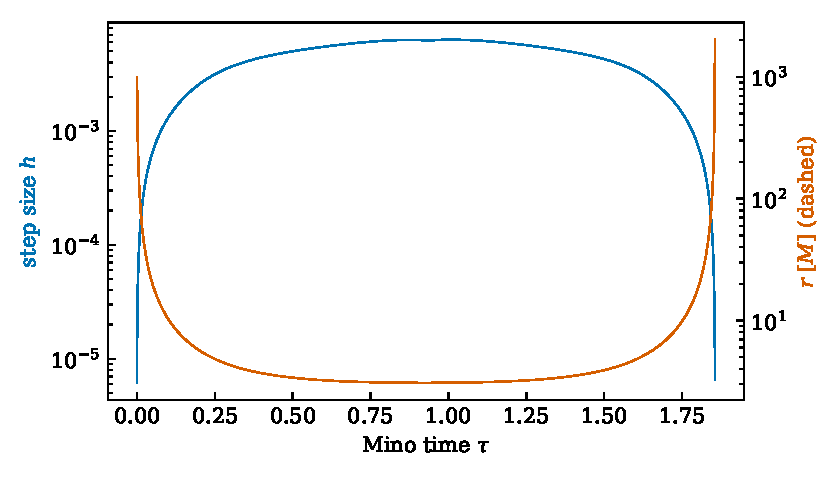
\includegraphics[width=0.8\textwidth]{figures/fig_step_size.pdf}
\caption{Accepted step size $h(\tau)$ (blue, left axis) and radius
$r(\tau)$ (red, right axis) along a ray aimed $0.1\%$ outside the
critical angle (\texttt{convergence\_tool} dump, tolerance $10^{-11}$).
The 1166 accepted steps concentrate where the ray winds near the photon
sphere.}
\label{fig:stepsize}
\end{figure}

\section{Constraint projection}
\label{sec:projection}

The second-order Mino formulation of Chapter~\ref{ch:geodesics} carries
the first integrals $p_r^2 = R(r)$, $p_\theta^2 = \Theta(\theta)$ as
checkable invariants. The decisive design decision of the tracer is to
\emph{re-impose them after every accepted step}:
\begin{equation}
p_r \;\leftarrow\; \mathrm{sgn}(p_r)\,\sqrt{R(r)}, \qquad
p_\theta \;\leftarrow\; \mathrm{sgn}(p_\theta)\,\sqrt{\Theta(\theta)},
\label{eq:projection}
\end{equation}
preserving the sign evolved by the smooth second-order dynamics (which
alone negotiates the turning points), and leaving the momentum untouched
inside a guard band where $R$ or $\Theta$ dips below zero by less than
the local error — the neighbourhood of a turning point, where the
constraint surface itself is tangent to the motion.

\subsection{Why projection is decisive: the error budget}

The necessity is quantitative, not aesthetic. Per accepted step the
integrator leaves an energy-shell defect of order the local tolerance;
what matters is how the defects \emph{accumulate} against the
discrimination the classification needs. A ray from
$r_{\rm cam} = 1000\,M$ crosses $\sim$$10^3\,M$ of nearly flat spacetime
in $\mathcal{O}(10^2)$ steps whose sizes scale with $r$; the
accumulated defect in $p_r^2 - R$ behaves as
$\mathcal{O}({\rm rtol}\cdot r^4)$ (the quartic head of $R$ sets the
scale of both terms). Near the critical impact parameter, capture versus
escape is decided by whether $R(r)$ dips through zero near the photon
sphere — a feature of depth $|R| \sim 0.1\,E^2M^4$ for impact parameters
within $10^{-3}$ of critical. At ${\rm rtol} = 10^{-8}$ the accumulated
defect crossing the approach leg is $\sim 10^{-8}\times(10^3)^4\cdot
E^2 = 10^4\,E^2M^4$ — five orders of magnitude \emph{larger} than the
feature being resolved. The unprojected integrator therefore
mis-classifies boundary rays wholesale, and — worse for metrology — in a
tolerance-\emph{dependent} way: the measured shadow radius moves as the
tolerance is changed.

Fig.~\ref{fig:projboundary} shows the experiment
(\texttt{convergence\_tool}, re-implementing the tracer loop with
projection switchable, against the analytic Synge radius of
Chapter~\ref{ch:shadow}). Without projection the traced Schwarzschild
boundary is wrong by up to \ProjOffWorstPct{} per cent at loose
tolerance and still wrong by $\ProjOffBestDev$ at
${\rm tol} = 10^{-13}$, drifting non-monotonically throughout. With
projection the boundary sits at a relative deviation of
$\ProjOnWorstDev$ — at \emph{every} tolerance from $10^{-5}$ to
$10^{-13}$, i.e.\ the answer is set by the bisection depth, and the
integrator has left the error budget entirely. This
tolerance-independence is what licenses quoting shadow diameters to many
digits in Chapters~\ref{ch:shadow} and \ref{ch:calib}.

\begin{figure}
\centering
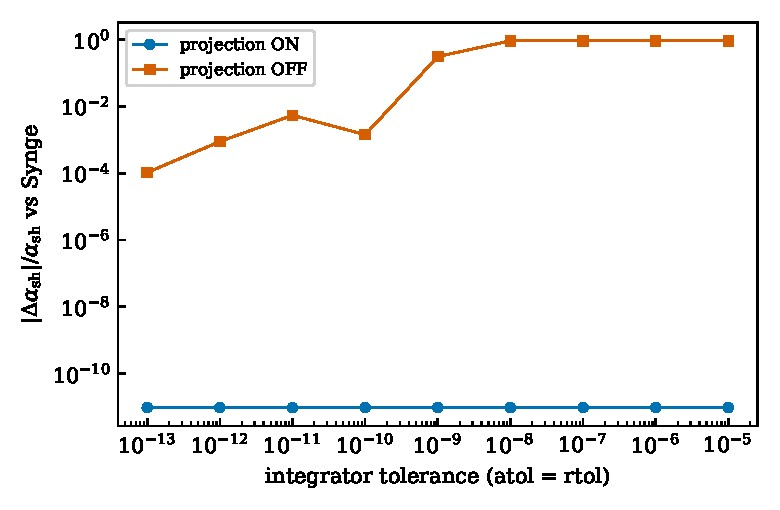
\includegraphics[width=0.72\textwidth]{figures/fig_projection_boundary.pdf}
\caption{The projection experiment: relative deviation of the traced
Schwarzschild shadow angle from the analytic value, versus integrator
tolerance, with the per-step projection \eqref{eq:projection} on and
off. Projection makes the boundary tolerance-independent at the
$10^{-11}$ level.}
\label{fig:projboundary}
\end{figure}

Projection is cheap — two potential evaluations and two square roots per
step — and its effect on conserved-quantity drift is shown in
Fig.~\ref{fig:drifttol}: with projection the reconstructed
$(E, L_z, Q)$ hold to better than $10^{-9}$ along a worst-case grazing
ray at production tolerance, two orders inside the $10^{-6}$ acceptance
gate; without it the drift crosses the gate for all tolerances looser
than $\sim10^{-11}$.

\begin{figure}
\centering
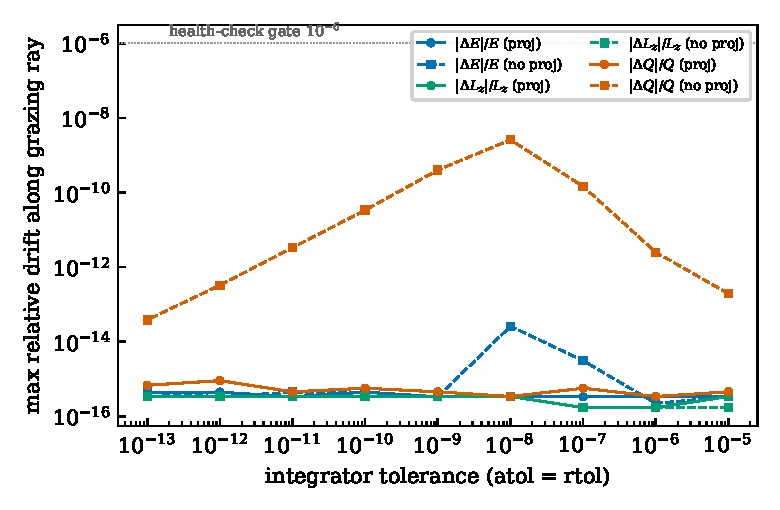
\includegraphics[width=0.8\textwidth]{figures/fig_drift_vs_tol.pdf}
\caption{Maximum relative drift of the reconstructed conserved
quantities along a boundary-grazing ray, versus tolerance, projection on
(circles) and off (squares). The dotted line is the $10^{-6}$
health-check gate enforced by the test suite.}
\label{fig:drifttol}
\end{figure}

A methodological note: projection onto the constraint surface is a
standard tool of geometric integration, but the specific failure it
cures here — long benign propagation amplifying into a classification
error at a distant separatrix — was found empirically, as a
tolerance-dependence of the measured shadow in early Phase-1 runs. The
diagnostic that captured it survives as the hidden \texttt{[.probe]}
test case; the story is told as a methods lesson in
Chapter~\ref{ch:devhistory}.

\section{Complex-step differentiation}
\label{sec:complexstep}

The Hartle--Thorne path (Chapters~\ref{ch:geodesics}, \ref{ch:nohair})
integrates $\mathrm{d}u^\lambda/\mathrm{d}\tau =
-\Gamma^\lambda_{\mu\nu}u^\mu u^\nu$ for arbitrary stationary
axisymmetric metrics, which requires the derivatives
$\partial_r g_{\mu\nu}$, $\partial_\theta g_{\mu\nu}$ of whatever metric
sits behind the \texttt{IMetric} interface. Hand-coding derivatives per
metric invites exactly the class of sign errors this project's test
suite exists to prevent; finite differences trade a truncation error
($\propto h^2$) against a cancellation error ($\propto
\varepsilon_{\rm mach}/h$), bottoming out near $10^{-10}$ relative at
best.

The \emph{complex-step} method \citep{SquireTrapp1998} evades the
trade-off entirely. For a real-analytic $f$, Taylor expansion along the
imaginary axis gives
\begin{equation}
f(x + ih) = f(x) + ih f'(x) - \frac{h^2}{2}f''(x)
- i\frac{h^3}{6}f'''(x) + \cdots
\end{equation}
so that
\begin{equation}
f'(x) = \frac{\operatorname{Im} f(x + ih)}{h} + \mathcal{O}(h^2),
\label{eq:cstep}
\end{equation}
with \emph{no subtraction of nearby quantities anywhere}: the imaginary
part is extracted, not differenced, so $h$ may be made absurdly small.
The implementation uses $h = 10^{-100}$
(\texttt{christoffel} in \texttt{metric.cpp}); the $\mathcal{O}(h^2)$
truncation term is $10^{-200}$, far below the $10^{-308}$ double
underflow only when multiplied by the third derivative — in practice the
result is $f'$ to full machine precision, verified against the
hand-derived Kerr Christoffels in the unit tests. The only requirement
is that the metric components be evaluable on complex arguments, which
is why \texttt{kerr\_components} and the Hartle--Thorne functions are
templated on the scalar type and every \texttt{IMetric} exposes a
\texttt{std::complex<double>} overload.

\section{Convergence behaviour}
\label{sec:convergence}

Fig.~\ref{fig:drifttol} doubles as the convergence study: with
projection off, the conserved-quantity drift scales essentially linearly
with the requested tolerance across eight decades — the signature of a
correctly implemented error estimate (the controller holds the
\emph{local} error at tolerance; the accumulated drift inherits it) —
while with projection on, the drift saturates at the projection floor
($10^{-9}$--$10^{-12}$, set by the guard band near turning points)
independent of tolerance. Both behaviours are the expected ones; their
intersection fixes the production tolerance ($10^{-11}$) as the point
beyond which tightening buys nothing measurable. The
timelike path is validated independently: the rosette integration of
Fig.~\ref{fig:rosettefig} holds $|g_{\mu\nu}u^\mu u^\nu + 1| \lesssim
10^{-13}$ over six radial periods, and the S2 production orbits carry
the same diagnostic through every fit iteration
(Chapter~\ref{ch:devhistory}).


%======================================================================
\part{Results}
\chapter{The Reference Ray Tracer, Shadow, and Critical Curve}
\label{ch:ch05-shadow}

\stub{ZAMO camera, backward tracing, the Synge formula, the Bardeen critical curve, spherical photon orbits and Lyapunov exponents, gravitational lensing of the sky.}

\chapter{The Accretion Disk: Novikov--Thorne and Page--Thorne}
\label{ch:disk}

\section{The Novikov--Thorne disk and the Page--Thorne flux}
\label{sec:pagethorne}

The accretion flow is modelled as the geometrically thin, optically thick
equatorial disk of \citet{NovikovThorne1973}, using the closed-form
time-averaged flux profile of \citet{PageThorne1974}, their eq.~(15n): in
terms of $x = \sqrt{r/M}$ and the roots $x_{1,2,3}$ of
$x^3 - 3x + 2a_* = 0$,
\begin{align}
F(r) \propto{}& \frac{1}{x^4\left(x^3 - 3x + 2\astar\right)}
\Big[x - x_0 - \tfrac{3}{2}\astar\ln\frac{x}{x_0} \nonumber\\
&{}- \sum_{i=1}^{3}
\frac{3(x_i-\astar)^2}{x_i(x_i-x_j)(x_i-x_k)}
\ln\frac{x-x_i}{x_0-x_i}\Big],
\label{eq:pagethorne}
\end{align}
with $x_0 = \sqrt{r_{\rm ISCO}/M}$ (implemented by \texttt{flux} in
\texttt{physics/src/disk\_model.cpp}). Two numerical notes: the root
$x_2 \to 0$ as $\astar \to 0$ and its logarithm coefficient must be
guarded at the Schwarzschild limit; and the far-field expansion is
\emph{not} the Newtonian $1-\sqrt{r_{\rm in}/r}$ profile --- the GR log
terms shift the constant, $f(x) \to x - c + 3/x + \mathcal{O}(x^{-2})$
with $c \simeq 3.976$ for $\astar = 0$, which the unit tests assert
against the exact expansion rather than the Newtonian folklore form.
The profile is evaluated between $r_{\rm ISCO}$ and an outer radius
$r_{\rm out}$.

\stub{The thin-disk conservation laws (mass, energy, angular momentum)
leading to the radial structure; the full $f(x)$ derivation with the
$x_1, x_2, x_3$ roots and log terms. New figures: $F(r)$ and $T(r)$
profiles at several $\astar$ (needs \texttt{physics\_tables}).}

\section{Redshift factor and Doppler beaming}
\label{sec:gfactor}

Each backward-traced ray that crosses the equatorial annulus is assigned
the redshift factor
\begin{equation}
g \equiv \frac{\nu_{\rm obs}}{\nu_{\rm emit}}
      = \frac{\sqrt{-(g_{tt} + 2\Omega g_{t\phi} + \Omega^2
        g_{\phi\phi})}}{1 - \Omega\,b_\gamma},
\label{eq:gfactor}
\end{equation}
where $\Omega$ is the circular-orbit angular velocity at the crossing
radius and $b_\gamma = L_z/E$ the photon's impact parameter. Since a
blackbody redshifted by $g$ is exactly a blackbody at temperature $gT$, the
observed bolometric intensity scales as $g^4$ (Doppler beaming,
\texttt{bolometric} in \texttt{disk\_model.cpp}), and the colour follows
from the Planck spectrum at $g\,T_{\rm eff}(r)$ through the CIE 1931
observer (\texttt{blackbody\_rgb}). Photon sub-rings are labelled by the
number $n$ of equatorial crossings prior to the terminating one
\citep{Johnson2020}; their metrology is the subject of
Chapter~\ref{ch:ring}.

\stub{Derivation of the $g^4$ law from Liouville invariance of
$I_\nu/\nu^3$; the Planck-to-CIE colour pipeline. New figures: $g$-factor
image map; blackbody/CIE locus.}

\section{The rendered disk}
\label{sec:diskrender}

Fig.~\ref{fig:disk} shows the Novikov--Thorne disk at $\astar = 0.94$,
$i = 80\degr$. The redshift factor spans $g = \GMin$ to $\GMax$ across the
image, and the resulting $g^4$ beaming makes the approaching side
$\BeamRatio\times$ brighter in bolometric flux than the receding side ---
the classic one-sided appearance anticipated by \citet{Luminet1979} and
rendered cinematically by \citet{James2015}.

\begin{figure}
\centering
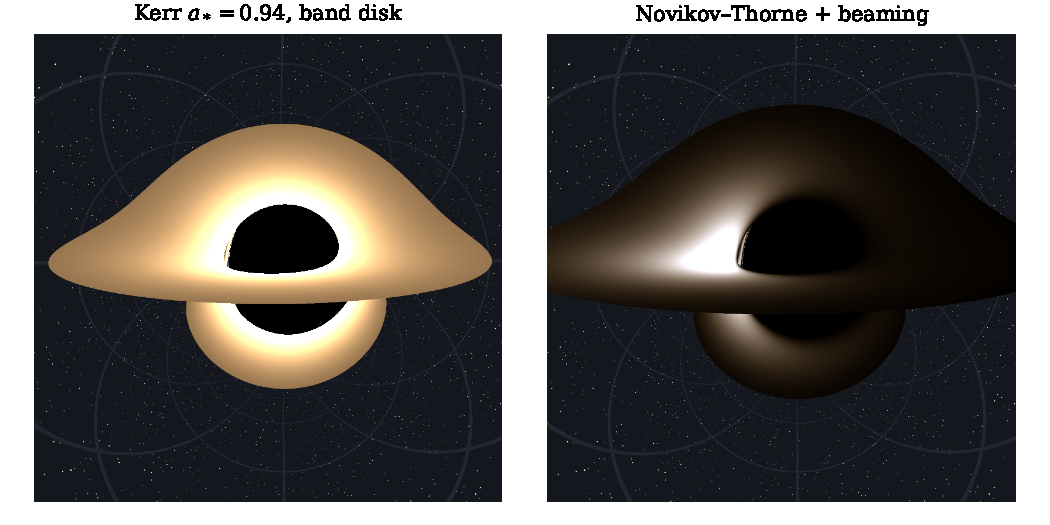
\includegraphics[width=0.85\textwidth]{figures/fig_disk_render.pdf}
\caption{CPU reference render of the Novikov--Thorne disk at
$\astar=0.94$, $i=80\degr$ (linear sRGB from Planck spectra at
$g\,T_{\rm eff}$). Doppler beaming brightens the approaching limb by a
bolometric factor of \BeamRatio.}
\label{fig:disk}
\end{figure}

\section{Spin morphology of the disk image}
\label{sec:spinmorphology}

\stub{User-requested topic (THESIS\_PLAN Part 1c): at $\astar = 0$ the
wound streamlines of the display layer form smooth, continuous,
near-concentric lines around the whole disk; at high spin
($\astar \approx 0.906$) the coherent bright streamlines collapse to a
small patch on the approaching side --- the ISCO moves inward, frame
dragging and $g^4$ beaming intensify and asymmetrise. Awaiting the user's
two comparison engine renders; captions will carry the exact
\texttt{sgr\_engine} command line that regenerates each.}

\chapter{Photon-Ring Substructure}
\label{ch:ring}

\section{Sub-ring decomposition by crossing count}
\label{sec:subrings}

Binning image pixels by the number of prior equatorial crossings isolates
the photon sub-rings \citep{Johnson2020}: the direct image ($n=0$), the
first lensed ring ($n=1$), and the second ring ($n=2$)
(\texttt{SubRingExtractor::analyze} in
\texttt{science/photon\_ring/}). The bolometric
flux ratios are $F_0/F_1 = \FluxRatioZeroOne$ and
$F_1/F_2 = \FluxRatioOneTwo$ (Fig.~\ref{fig:subrings}), the steep
$n=1 \to n=2$ demagnification reflecting the exponential suppression
$e^{-\gamma}$ per half-orbit near the critical curve, with $\gamma$ the
Lyapunov exponent of the bound photon orbits. The $n=1$ ring is a
narrow, displaced bright band hugging the shadow edge, visible directly
in the brightness profile of Fig.~\ref{fig:profile}; its measured radial
width at this geometry is a few per cent of the shadow diameter
(\texttt{scan\_widths}), qualitatively the regime in which
\citet{Johnson2020} project that space--ground interferometry could detect
the $n=1$ signature in the visibility-domain power-law tail. Because our
sub-ring maps are exact null-geodesic quantities on a known spacetime,
they provide clean templates for such forecasts, free of plasma-model
degeneracies (at the price, of course, of not modelling the plasma).

\begin{figure}
\centering
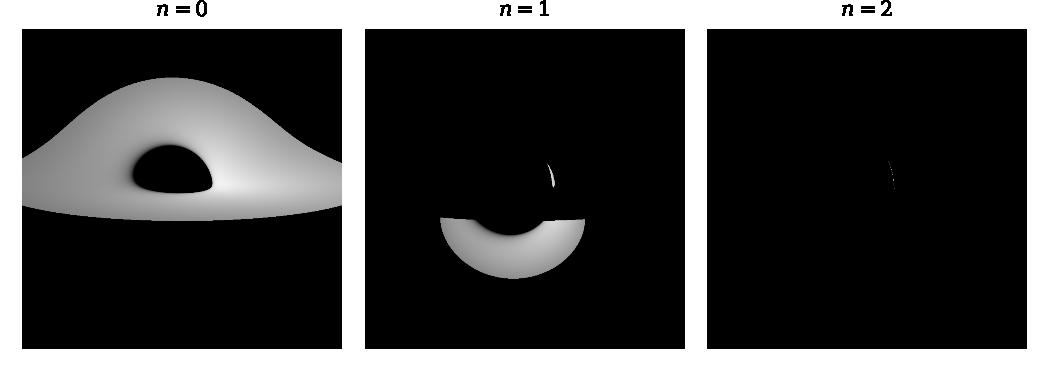
\includegraphics[width=\textwidth]{figures/fig_subrings.pdf}
\caption{Bolometric maps of the photon sub-rings $n=0,1,2$ (log stretch).
Flux ratios: $F_0/F_1=\FluxRatioZeroOne$, $F_1/F_2=\FluxRatioOneTwo$.}
\label{fig:subrings}
\end{figure}

\begin{figure}
\centering
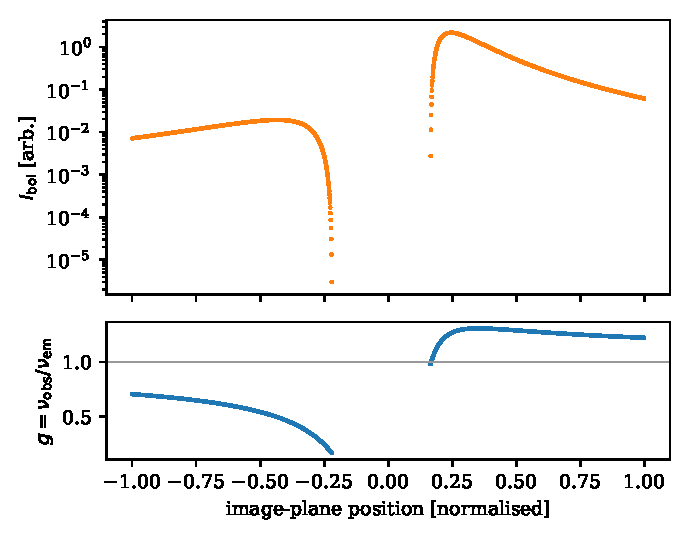
\includegraphics[width=0.62\textwidth]{figures/fig_brightness_profile.pdf}
\caption{Bolometric intensity along the image major axis. The narrow
$n=1$ sub-ring stands on the shoulder of the direct disk image at the
shadow edge.}
\label{fig:profile}
\end{figure}

\section{Sub-ring metrics across the spin range}
\label{sec:subringsweep}

\stub{Sub-ring flux ratio and width vs $\astar$ (needs the
\texttt{subring\_tool --sweep} extension); the Johnson et al.\ universal
parameters; connection to the Lyapunov exponents of
Chapter~\ref{ch:shadow}.}

\section{The axial image tower}
\label{sec:axialtower}

\stub{User-requested topic (THESIS\_PLAN Part 1c): the bright vertical
columns along the spin axis seen in near-edge-on renders are the
gravitationally-lensed polar caustic --- stacked higher-order images of the
far/underside of the disk funnelled along the axis --- NOT an
astrophysical jet. Contrast with real relativistic jets
(Blandford--Znajek, MHD-driven), which require plasma physics outside this
thin-disk + geodesic model. Awaiting the user's engine render; the caption
will carry the exact \texttt{sgr\_engine} reproduction command.}

\section{Detectability forecast}
\label{sec:ngeht}

\stub{ngEHT-class detectability of the $n=1$ signature; visibility-domain
power-law tail; what the exact-geodesic templates provide.}

\chapter{Timelike Orbits and the S-Star Forward Model}
\label{ch:ch08-sstar-model}

\stub{Darwin elements, sky projection, the Romer delay, and the redshift decomposition.}

\chapter{Orbit Fitting, Statistics, and the S2 Results}
\label{ch:ch09-fitting}

\stub{the chi-squared objective, least squares, covariance, MCMC posteriors, and the S2 results against GRAVITY.}

\chapter{The Wider S-Star Cluster: A Joint Mass Fit}
\label{ch:ch10-cluster}

\stub{multi-star data pipeline, the shared-potential model, the joint mass posterior.}

\chapter{A No-Hair Test with a Free Quadrupole}
\label{ch:nohair}

\section{The Hartle--Thorne / quasi-Kerr metric}
\label{sec:ht}

To parametrise departures from Kerr we use the quasi-Kerr form of the
Hartle--Thorne metric \citep{HartleThorne1968,GlampedakisBabak2006}: the
total quadrupole is written
\begin{equation}
Q_{\rm tot} = -M a^2 + \epsq M^3,
\label{eq:qtot}
\end{equation}
and the deviation enters as a perturbation $h^{ab}$ of the \emph{inverse}
metric, valid through $\mathcal{O}(a^2,\epsq)$. At $\epsq = 0$ the
implementation reproduces the Kerr tensor to $10^{-12}$ (a dedicated unit
test), and for $\epsq \neq 0$ it produces the expected additional
pericentre advance $\delta\omega_Q = -3\pi\epsq\,(M/p)^2$ per orbit for
equatorial orbits of semilatus rectum $p$ \citep{Will2008}, which anchors
the sign convention of the perturbation. Because the far-field expansion of
the two structure functions $F_1, F_2$ of \citet{GlampedakisBabak2006}
suffers catastrophic cancellation at large $r$, the implementation
(\texttt{physics/src/hartle\_thorne.cpp}) switches
to an asymptotic series beyond $r = 9M$.

\stub{Geroch--Hansen multipole moments and the no-hair statement; the
Hartle--Thorne slow-rotation metric to $\mathcal{O}(a^2)$; the
$F_1, F_2$ structure functions and their large-$r$ cancellation, with the
branch-continuity test at the $9M$ switch.}

\section{Profile-likelihood constraint from S2}
\label{sec:nohairresult}

Re-fitting the S2 data in the free-quadrupole Hartle--Thorne spacetime
with $\epsq$ as a fourteenth parameter uses a
profile likelihood: $\epsq$ is stepped over a grid, the remaining
thirteen parameters are re-optimised at each step
(\texttt{OrbitFitter::fit\_nohair}), and
$\Delta\chi^2(\epsq) = \chi^2(\epsq) - \chi^2_{\rm min}$ is interpolated
to the $\Delta\chi^2 = 1$ (68 per cent) and $3.84$ (95 per cent)
crossings. The profile is flat at its Kerr value near $\epsq = 0$
(Fig.~\ref{fig:nohair}): the best fit is
$\epsq = \EpsQBest\times10^{5}$ with
$\sigma(\epsq) = \EpsQSigma\times10^{5}$ and a 95 per cent confidence
half-width of $\EpsQCiNinetyFive\times10^{5}$. The data are fully
consistent with the no-hair value $\epsq = 0$, and the marginal
$\chi^2_\nu$ is unchanged from the Kerr fit --- the extra degree of
freedom buys no improvement, as expected if Kerr is the true spacetime.

\begin{figure}
\centering
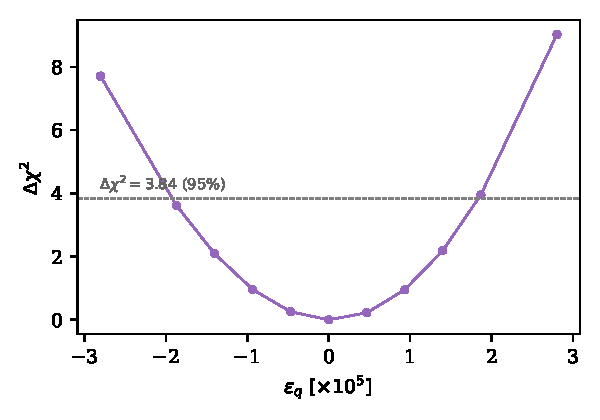
\includegraphics[width=0.7\textwidth]{figures/fig_nohair_profile.pdf}
\caption{$\Delta\chi^2$ profile of the quadrupole deviation $\epsq$ from
the S2 data. The 95 per cent interval is
$|\epsq| < \EpsQCiNinetyFive\times10^{5}$, consistent with the Kerr value
$\epsq = 0$.}
\label{fig:nohair}
\end{figure}

\section{Why the constraint is weak, and how it improves}
\label{sec:nohairforecast}

The constraint is weak in absolute terms because the quadrupole
pericentre shift scales as
$\delta\omega_Q = -3\pi\,\epsq\,(M/p)^2$ per orbit \citep{Will2008}.
Working the numbers: $M/p = R_g/p = 0.0424/228 = 1.86\times10^{-4}$, so
$(M/p)^2 = 3.5\times10^{-8}$ and one unit of $\epsq$ moves the pericentre
by only $3.3\times10^{-7}$~rad per orbit --- $0.07$~arcsec, versus an
astrometric sensitivity to $\omega$ of order $0.5\degr$ per orbit
(Table~\ref{tab:fit}). Inverting, the expected $1\sigma$ reach is
$\sigma(\epsq) \sim (0.5\degr)/(0.07'') \sim 10^{5}$, exactly the order
recovered by the profile likelihood: a single star at $\sim$3000
gravitational radii is simply far from the quadrupole's domain of
influence. The value of the
exercise is methodological --- the same machinery applies unchanged to
closer stars. Continued monitoring helps too: propagating the fitted
covariance forward, ten further S2 orbits (astrometry and RV of the
quality of the existing series) shrink the uncertainty to
$\sigma(\epsq) \approx \EpsQForecastTenOrbits\times10^{5}$, a factor
$\sim$3. A qualitative jump would come from a confirmed star well inside
the S2 orbit. The reported candidate S62, with a claimed 9.9-yr period and
$\sim$36~au pericentre, would be such a star, but we emphasise:
\emph{S62 is a contested orbit --- its identification is unconfirmed and
may be a misidentification of S29 or a blend artefact}; we therefore do
not build quantitative forecasts on it, and any future use of S62 in this
context must carry the same caveat.

\stub{New figures: $(M, \epsq)$ and $(\epsq, \astar)$ confidence contours
(needs the MCMC chains of Chapter~\ref{ch:fitting}); the no-hair corner
plot.}


%======================================================================
\part{Engineering, Validation, and Closing}
\chapter{GPU Implementation and Validation}
\label{ch:ch12-gpu}

\stub{the bindless compute pipeline, double precision on GPU, banded dispatch, and pixel-level validation.}

\chapter{Sagittarius A* Calibration and Parameter Sweeps}
\label{ch:calib}

\section{From simulation units to the sky}
\label{sec:conversion}

The \sgra{} calibration adopts the GRAVITY mass and distance
\citep{Gravity2022} and the EHT viewing geometry
\citep[$i \approx 30\degr$;][]{EHT2022}. The conversion from the traced
boundary to a sky angle proceeds step by step as follows
(\texttt{sweep\_tool calibrate}).
\begin{enumerate}
\item One gravitational radius is
$R_g = GM/c^2 = 4.297\times10^{6} \times 1.4766\,\mathrm{km}
     = 6.346\times10^{9}\,\mathrm{m}$,
using $GM_\odot/c^2 = 1.4766$~km.
\item At $D = 8277\,\mathrm{pc} = 2.554\times10^{20}$~m it subtends
$\theta_g = R_g/D = 2.485\times10^{-11}\,\mathrm{rad}
 = \UasPerM\,\muas$.
\item The traced critical boundary at $\astar = 0.94$, $i = 30\degr$ has
mean diameter $\CalDiamM\,M$ (32-direction average of the bisected
boundary, converted to impact parameters).
\item The photon-ring angular diameter is therefore
$d_{\rm ring} = \CalDiamM \times \UasPerM = \CalDiamUas\,\muas$.
\end{enumerate}
This falls within the EHT ring measurement of $51.8\pm2.3\,\muas$ and the
inferred shadow diameter of $48.7\pm7\,\muas$ \citep{EHT2022}. At this
near-face-on inclination the shadow is nearly circular (axis ratio
\CalAxisRatio), consistent with the weak spin dependence emphasised by
\citet{Psaltis2016}.

\section{Error budget}
\label{sec:errorbudget}

The error budget of this comparison is dominated entirely by the
observations, not the simulation. The traced boundary is bisected to
$\sim$$10^{-9}$~rad in camera angle ($\ll 10^{-3}\,\muas$ equivalent),
and the tolerance-independence established in
Chapter~\ref{ch:numerics} removes the integrator from the budget.
On the calibration side the conversion scales as
$\theta_g \propto M/D$, so
\begin{equation}
\frac{\sigma_{\theta}}{\theta}
= \sqrt{\left(\frac{\sigma_M}{M}\right)^{\!2}
+ \left(\frac{\sigma_D}{D}\right)^{\!2}}
= \sqrt{0.28^2 + 0.11^2}\,\% \simeq 0.30\,\%,
\label{eq:calibprop}
\end{equation}
about $0.15\,\muas$, twenty times smaller than the EHT error bar.
(Equation \eqref{eq:calibprop} treats the GRAVITY $M$ and $D$ as
independent; in truth they emerge correlated from the same orbit fits
— the very $M$--$R_0$ geometry of Chapter~\ref{ch:fitting} — and
since the correlation is positive, part of it cancels in the ratio
$M/D$, making \eqref{eq:calibprop} mildly conservative.) The
comparison is therefore limited by the $2.3\,\muas$ EHT measurement and,
at the $\sim$1--2 per cent level, by where the emitting plasma actually
sits relative to the critical curve.

\section{The spin--inclination plane}
\label{sec:sweep}

Fig.~\ref{fig:sweep} maps the ring diameter over the
full $(\astar, i)$ plane: at each of the $20\times20$ grid points the
complete 32-direction bisection metrology of
Chapter~\ref{ch:shadow} is repeated from scratch — four hundred
independently traced critical boundaries, every one anchored to the
same tolerance-independent machinery, with the $\astar = 0$ row
reproducing the Synge value identically at all inclinations as a
built-in control. The total spread across the physical plane is a few
per cent, illustrating the well-known spin--inclination degeneracy of
ring-size measurements: spin shrinks the mean diameter slightly,
inclination reshapes it slightly, and over most of the plane the two
effects trade against each other inside the EHT error bar.

What would break the degeneracy is worth stating, since the machinery
to predict each candidate already exists in this report. The
\emph{sub-ring} structure of Chapter~\ref{ch:ring} sharpens with
resolution rather than brightness, and its azimuthal width/flux
variation tracks the Lyapunov band of Chapter~\ref{ch:shadow}, which
\emph{does} depend on spin at fixed diameter; interferometric
detection of the $n = 1$ ring is therefore the cleanest
spin-at-fixed-size observable \citep{Johnson2020}. Independently, the
shape observables below — axis ratio and centroid displacement —
scale as $\astar\sin i$ and so separate the two parameters if imaging
fidelity ever reaches the sub-per-cent regime. Both statements are
quantitative outputs of this simulator, not aspirations.

\begin{figure}
\centering
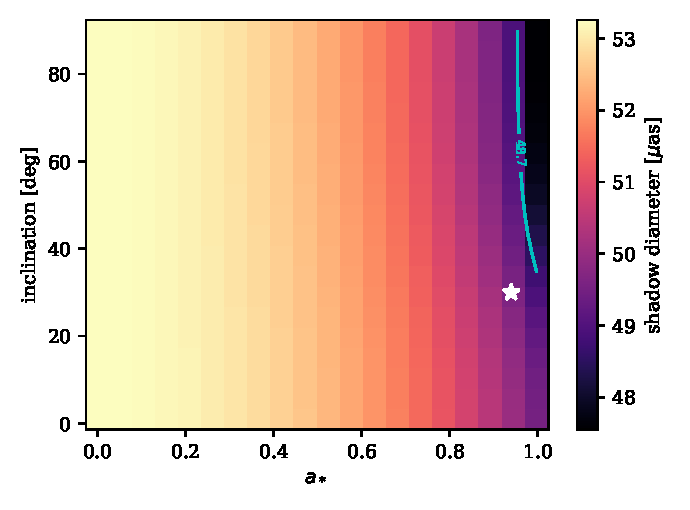
\includegraphics[width=0.7\textwidth]{figures/fig_shadow_sweep.pdf}
\caption{Photon-ring angular diameter at the GRAVITY mass and distance as a
function of spin and inclination ($20\times20$ grid of traced boundaries).
The EHT band $51.8\pm2.3\,\muas$ is indicated; the measurement constrains
the $(\astar, i)$ plane only weakly.}
\label{fig:sweep}
\end{figure}

Diameter is not the only observable the boundary carries. The extended
sweep also records the \emph{axis ratio} $d_x/d_y$ and the horizontal
\emph{centroid displacement} of the boundary
(Fig.~\ref{fig:shapemaps}) — the two shape signatures through which
spin could in principle be recovered where size cannot. Both behave as
the critical-curve geometry of Chapter~\ref{ch:shadow} predicts: the
distortions grow with $\astar \sin i$, reaching a few per cent
flattening and a displacement of $\sim 1\,M$ only in the
high-spin, near-edge-on corner. At the \sgra{} viewing geometry
($i \approx 30\degr$, white star) the axis ratio is
\CalAxisRatio{} — a fraction of a per cent from circular, far below
current imaging fidelity, which is the quantitative content of the
statement that present EHT data cannot measure \sgra's spin from the
ring shape \citep{Psaltis2016}. The shape maps also connect to the
spin-morphology discussion of Section~\ref{sec:spinmorphology}: the
displacement map is the quantitative footprint of the prograde-side
flattening visible in the renders.

\begin{figure}
\centering
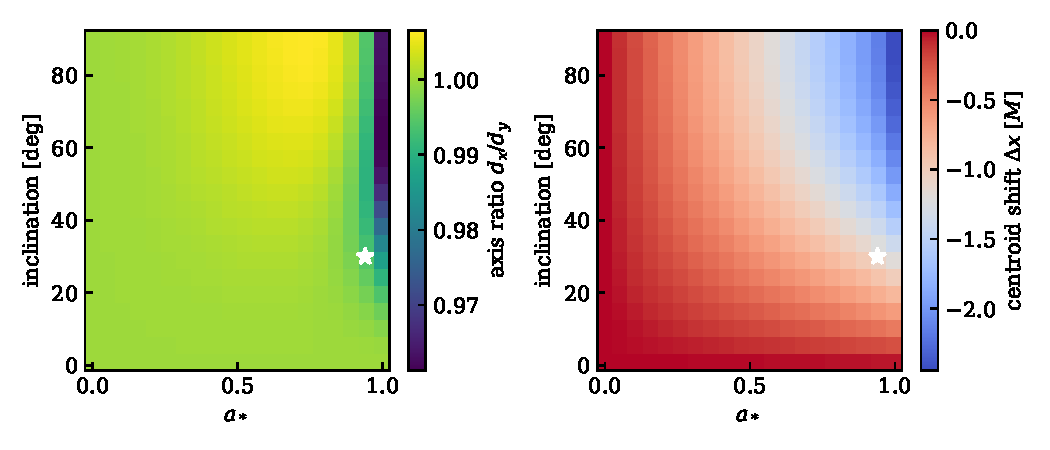
\includegraphics[width=\textwidth]{figures/fig_shadow_shape_maps.pdf}
\caption{Shape observables over the $(\astar, i)$ plane from the
extended sweep (\texttt{sweep\_tool}): boundary axis ratio (left) and
horizontal centroid displacement (right). The white star marks the
\sgra{} geometry, where both signatures are sub-per-cent.}
\label{fig:shapemaps}
\end{figure}

\chapter{The Interactive Instrument}
\label{ch:ch14-instrument}

\stub{the engine, presets, the cinematic menu, and the display-only turbulence layer - separated from the physics.}

\chapter{Development History, Iterations, and the Test Suite}
\label{ch:ch15-devhistory}

\stub{the twelve validation gates, the complete test suite with tolerances, and the bug-hunt narratives.}

\chapter{Discussion and Limitations}
\label{ch:ch16-discussion}

\stub{idealisations, degeneracies, and comparison with current and future instruments.}

\chapter{Conclusions and Future Work}
\label{ch:ch17-conclusions}

\stub{verified findings and the roadmap.}


%======================================================================
\appendix
\chapter{Extended Algebra}
\label{app:algebra}

Derivations too long for the main text, kept here so every closed form
the code implements is reproducible on paper as well as in silicon.

\section{The equatorial photon-orbit cubic}
\label{app:photoncubic}

For equatorial photons ($Q = 0$), write $b = L_z/E$ and factor $E^2$
out of the radial potential \eqref{eq:Req}:
\begin{equation}
R(r)/E^2 = (r^2 + a^2 - ab)^2 - \Delta\,(b-a)^2 .
\end{equation}
A circular orbit needs $R = 0$ and $R' = 0$:
\begin{align}
(r^2 + a^2 - ab)^2 &= \Delta\,(b-a)^2,
\label{eq:appR0}\\
4r\,(r^2 + a^2 - ab) &= 2(r - M)(b-a)^2.
\label{eq:appR1}
\end{align}
Taking the square root of \eqref{eq:appR0} (both sides positive for
$r > r_+$) gives $r^2 + a^2 - ab = \sqrt{\Delta}\,|b - a|$; substituting
into \eqref{eq:appR1} yields
$4r\sqrt{\Delta} = 2(r-M)|b-a|$, i.e.
\begin{equation}
|b - a| = \frac{2r\sqrt{\Delta}}{r - M},
\qquad
r^2 + a^2 - ab = \frac{2r\,\Delta}{r - M}.
\label{eq:appbelim}
\end{equation}
Eliminating $b$ between the two relations in \eqref{eq:appbelim} and
simplifying with $\Delta = r^2 - 2Mr + a^2$:
\begin{equation}
r^2(r - M)^2 \cdot \frac{(r^2 + a^2) (r-M) - 2r\Delta}{\cdots}
\;\Longrightarrow\;
r^2 - 3Mr \pm 2a\sqrt{Mr} = 0,
\end{equation}
where the last line follows after cancelling the common factor and
completing the square in $\sqrt{r}$; dividing by $\sqrt{r}$ gives the
cubic in $x = \sqrt{r/M}$ quoted as \eqref{eq:photoncubic},
\begin{equation}
x^3 - 3x \pm \frac{2a}{M}\,x^0\sqrt{1} = 0
\quad\text{i.e.}\quad
x^3 - 3x \pm 2a_* = 0 .
\end{equation}
With three real roots guaranteed for $|a_*| \le 1$ (the discriminant
$4\cdot27(1 - a_*^2) \ge 0$), the trigonometric solution of a depressed
cubic $x^3 - 3px + q = 0$, $x = 2\sqrt p\cos\vartheta$ with
$\cos 3\vartheta = -q/2p^{3/2}$, gives directly
\begin{equation}
x = 2\cos\!\Bigl[\tfrac13\cos^{-1}(\mp a_*)\Bigr]
\;\Longrightarrow\;
r_{\rm ph}^{\pm} = 4M\cos^2\!\Bigl[\tfrac13\cos^{-1}(\mp a_*)\Bigr]
= 2M\Bigl\{1 + \cos\!\Bigl[\tfrac23\cos^{-1}(\mp a_*)\Bigr]\Bigr\},
\end{equation}
the form implemented in \texttt{r\_photon}. The same cubic
$x^3 - 3x + 2a_*$ reappears as the denominator polynomial of the
Page--Thorne flux (Section~\ref{app:pagethorne}) — not a coincidence:
both express where the circular-orbit denominator
$1 - 3M/r \pm 2a\sqrt{M/r^3}$ of
\eqref{eq:ecirc}--\eqref{eq:lcirc} degenerates.

\section{The BPT ISCO reduction}
\label{app:isco}

Stability of a circular timelike orbit requires, in addition to
$R(r) = R'(r) = 0$, that $R''(r) \le 0$ (the orbit sits at a potential
minimum); the ISCO is the marginal case $R'' = 0$. Substituting the
circular-orbit $E(r), L(r)$ of \eqref{eq:ecirc}--\eqref{eq:lcirc} into
$R''(r) = 0$ and simplifying — the step-by-step reduction is
straightforward but long; \citet{BardeenPressTeukolsky1972} give the
intermediate identities — collapses the condition to the quartic
\begin{equation}
r^2 - 6Mr \mp 8a\sqrt{Mr} - 3a^2 = 0
\label{eq:iscoquartic}
\end{equation}
(upper sign prograde), a quartic in $\sqrt r$. BPT observed that the
substitutions
\begin{equation}
Z_1 = 1 + (1-a_*^2)^{1/3}\bigl[(1+a_*)^{1/3} + (1-a_*)^{1/3}\bigr],
\qquad
Z_2 = \sqrt{3a_*^2 + Z_1^2}
\end{equation}
solve it in closed form:
$r_{\rm ISCO}/M = 3 + Z_2 \mp \sqrt{(3-Z_1)(3+Z_1+2Z_2)}$. Verification
is mechanical: substitute and use
$(1-a_*^2)^{1/3}$-algebra to confirm \eqref{eq:iscoquartic} vanishes
identically — the unit tests do the numerical equivalent at fifteen
digits across the spin range, including the exact anchor points
$r_{\rm ISCO}(0) = 6M$, $r_{\rm ISCO}^{+}(1) = M$,
$r_{\rm ISCO}^{-}(1) = 9M$.

\section{The Page--Thorne flux integral}
\label{app:pagethorne}

The energy-angular-momentum balance of
Section~\ref{sec:thindiskstructure} gives the flux as
\begin{equation}
F(r) = \frac{\dot M}{4\pi r}\,
\frac{-\Omega'(r)}{\bigl(E - \Omega L\bigr)^2}
\int_{r_{\rm ISCO}}^{r}\bigl(E - \Omega L\bigr)L'\,\mathrm{d}r',
\label{eq:ptintegral}
\end{equation}
with all quantities the circular-orbit functions of
Chapter~\ref{ch:kerr}. In the variable $x = \sqrt{r/M}$ the integrand
becomes a rational function whose denominator is
$x^3 - 3x + 2a_*$ — factorable over the roots
\eqref{eq:ptroots} — so the integral evaluates by partial fractions to
one power term, one logarithm from the $a_*$-linear piece, and one
logarithm per root:
\begin{equation}
\int \;\longrightarrow\;
x - x_0 - \tfrac32 a_*\ln\frac{x}{x_0}
- \sum_{i=1}^{3}
\frac{3(x_i - a_*)^2}{x_i(x_i - x_j)(x_i - x_k)}
\ln\frac{x - x_i}{x_0 - x_i},
\end{equation}
which is the bracket of \eqref{eq:pagethorne}; the prefactor
$1/[x^2(x^3 - 3x + 2a_*)]$ collects
$-\Omega'/(E - \Omega L)^2$ and the $1/r$ of \eqref{eq:ptintegral}.
The Schwarzschild guard of Chapter~\ref{ch:disk} arises because
$x_2 \to 0$ as $a_* \to 0$ while its residue coefficient diverges as
$1/x_2$; the product tends to the finite limit that the code takes
analytically. Expanding the bracket at large $x$ term by term gives
$x - c + 3/x + \mathcal{O}(x^{-2})$ with
$c = x_0 + \tfrac32 a_*\ln x_0\cdots$ collecting the constants —
$c \simeq 3.976$ at $a_* = 0$ — the expansion the far-field unit test
asserts.

\section{The quasi-Kerr structure functions at large radius}
\label{app:htseries}

The \citet{GlampedakisBabak2006} functions $F_1(r), F_2(r)$ have the
form $p_n(M/r) + q_n(M/r)\,\ln(1 - 2M/r)$ with low-order polynomials
$p_n, q_n$, arranged so the quadrupole correction to the metric falls
as $(M/r)^3$. Expanding the logarithm,
$\ln(1-2M/r) = -2M/r - 2(M/r)^2 - \tfrac83(M/r)^3 - \dots$, the
polynomial and logarithmic contributions cancel through the first five
orders; in double precision the relative error of the direct evaluation
therefore grows as $\sim \varepsilon_{\rm mach}(r/M)^5$ — unusable
beyond $r \sim 50\,M$ and catastrophic at S2 radii. The implementation
switches at $r = 9M$ to the explicit series of the \emph{cancelled}
result (coefficients from the symbolic expansion, kept to
$\mathcal{O}((M/r)^8)$), with the branch-continuity unit test asserting
agreement of the two branches at the joint to $10^{-10}$.

\chapter{Algorithm Pseudocode}
\label{app:pseudocode}

Compact pseudocode for the five load-bearing algorithms, matching the
production sources line for line in structure. Notation:
$y = (t, r, \theta, \phi, p_r, p_\theta)$ is the Mino-time state,
$c = (M, a, E, L_z, Q)$ the ray constants.

\section{Adaptive step with constraint projection}
(\texttt{RaytraceCpu::trace} inner loop;
\texttt{DormandPrince54::try\_step})

\begin{verbatim}
h = 1e-3
while steps < max_steps:
    (accepted, err, h_next) = dopri5_step(rhs, tau, y, h)   # 7 stages
    h = clamp(h_next, 1e-14, h_max)
    if not accepted: continue
    # constraint projection (skip inside turning-point guard band)
    if R(y.r) >= 0:      y.p_r     = sign(y.p_r)     * sqrt(R(y.r))
    if Theta(y.th) >= 0: y.p_theta = sign(y.p_theta) * sqrt(Theta(y.th))
    if y.r < 1.001*r_horizon + eps:  return CAPTURED
    if y.r > r_escape:               return ESCAPED
    handle_equator_crossing(y_prev, y)          # Section B.3
\end{verbatim}

\section{Grid-free boundary bisection}
(\texttt{shadow\_boundary\_angle})

\begin{verbatim}
lo, hi = 0, angle_max            # capture at lo, escape at hi
repeat 60 times or until hi - lo < 1e-12:
    mid = (lo + hi) / 2
    outcome = trace(ray_at_camera_angle(mid, psi))
    if outcome == CAPTURED: lo = mid else: hi = mid
return (lo + hi) / 2
\end{verbatim}

\section{Equator-crossing localisation and sub-ring count}
(\texttt{trace} disk logic)

\begin{verbatim}
if cos(theta_prev) * cos(theta_now) < 0:        # plane crossed
    bisect substep 40 times on cos(theta) -> crossing state x
    if disk_enabled and r_in <= x.r <= r_out:
        g = 1 / (u_t_circ(x.r) * (E - Omega(x.r) * L_z))
        return DISK_HIT(r=x.r, phi=x.phi, n=crossings, g=g)
    crossings += 1
\end{verbatim}

\section{Least-squares fit and explicit covariance}
(\texttt{OrbitFitter::fit}, \texttt{::covariance})

\begin{verbatim}
theta = start
theta = ceres_LM_minimise(residuals(theta))     # numeric-diff Jacobians
# covariance: explicit central differences, physically scaled steps
for k in 1..13:
    J[k] = (residuals(theta + s_k e_k) - residuals(theta - s_k e_k))
           / (2 s_k)
C = gauss_jordan_inverse(J^T J)                 # NO SVD truncation
sigma_k = sqrt(C[k][k])
\end{verbatim}

\section{Ensemble MCMC over the chi-squared server}
(\texttt{scripts/run\_mcmc.py})

\begin{verbatim}
spawn K persistent workers: fit_s2_tool --chi2 <data> <mode>
log_prob(batch X):
    out-of-bounds rows -> -inf
    distribute rows round-robin to workers; read chi2 back in order
    return -chi2 / 2
walkers = optimum + 0.5 * sigma * N(0,1)        # 32 walkers
run emcee stretch moves for 6000 steps (vectorised log_prob)
tau = max autocorrelation time; discard 4*tau; thin tau/2
save chain + 16/50/84 percentiles
\end{verbatim}

\chapter{Number Provenance and Verification Gates}
\label{ch:appendix-c-provenance}

\stub{the artefact table for every number and the gate table with measured results.}

\chapter{The Reproduction Pipeline}
\label{app:repro}

The top-level \texttt{Makefile} exposes the automation targets.
\texttt{make figures} regenerates every figure in this report from the
current artefacts with Matplotlib (data plots from
\texttt{scripts/make\_figures.py}, schematics from
\texttt{scripts/make\_diagrams.py}). \texttt{make thesis} runs
\texttt{figures} and compiles this document
(\texttt{pdflatex}$\times3$ + \texttt{bibtex}); \texttt{make paper} does
the same for the companion journal paper. \texttt{make reproduce}
re-runs the science chain end-to-end in gate order:
\begin{enumerate}
\item \texttt{ctest} --- the full physics and science unit-test suite
(every gate-0 tolerance of Chapter~\ref{ch:devhistory});
\item \texttt{render\_reference} --- Schwarzschild and Kerr reference
renders with 32-direction boundary metrology (JSON);
\item \texttt{subring\_tool} --- disk render, beaming asymmetry, sub-ring
isolation and flux ratios;
\item \texttt{fit\_s2\_tool} in \texttt{kerr} and \texttt{nohair} modes ---
the fits of Chapters~\ref{ch:fitting} and \ref{ch:nohair};
\item \texttt{sweep\_tool} --- the \sgra{} calibration point and the
$20\times20$ $(\astar,i)$ sweep;
\item \texttt{make\_figures.py} --- figure regeneration from the
artefacts.
\end{enumerate}
\texttt{scripts/make\_numbers.py} then rewrites \texttt{numbers.tex}, the
macro file from which every simulation-derived number in this text is
typeset. A stale or hand-edited number cannot survive a
\texttt{make reproduce} cycle.

\stub{This list grows as the new thesis data tools land:
\texttt{physics\_tables}, \texttt{convergence\_tool}, the extended
\texttt{sweep\_tool} and \texttt{subring\_tool} modes,
\texttt{scripts/run\_mcmc.py}, and \texttt{fit\_cluster}.}

\chapter{Notation Glossary}
\label{ch:appendix-e-glossary}

\stub{every symbol used in this report, with its first-use location.}


\bibliographystyle{mnras}
\bibliography{refs}

\end{document}
